% TODO: Tout récrire:
% Section:
% Applications (instructables et spot welder (ça explique pk)
% Condensateur diélectrique
% Super condensateur

% a4paper, legalpaper ou letterpaper
\documentclass[12 pt, a4paper]{report} % article, book or report
\usepackage[utf8]{inputenc}
\usepackage[T1]{fontenc}
\usepackage{hyperref}
\usepackage{todonotes}
\usepackage{gensymb} % superscript
\usepackage{textcomp} % superscript
\usepackage{amsmath} % symboles des degrés

% --------------------  NOMBRES ET UNITÉS ---------------------------
\usepackage{siunitx}
\iffalse % explication des fonctions courantes
The package provides the user macros:
• \ang[hoptionsi]{hanglei}
• \num[hoptionsi]{hnumberi}
• \si[hoptionsi]{huniti}
• \SI[hoptionsi]{hnumberi}[hpre-uniti]{huniti}
• \numlist[hoptionsi]{hnumbersi}
• \numrange[hoptionsi]{hnumbersi}{hnumber2i}
• \SIlist[hoptionsi]{hnumbersi}{huniti}
• \SIrange[hoptionsi]{hnumber1i}{hnumber2i}{huniti}
• \sisetup{hoptionsi}
• \tablenum[hoptionsi]{hnumberi}
plus the S and s column types for decimal alignments and units in tabular environments.
12 345.678 90        \num{12345,67890}
1 ± 2i               \num{1+-2i}
0.3 × 1045           \num{.3e45}
1.654 × 2.34 × 3.430 \num{1.654 x 2.34 x 3.430}

\si{kg.m.s^{-1}}
kg m s−1
Simple lists and ranges of numbers can be handled.
\numlist{10;20;30} \\
\SIlist{0.13;0.67;0.80}{\milli\metre} \\
\numrange{10}{20} \\
\SIrange{0.13}{0.67}{\milli\metre}
10, 20 and 30
0.13 mm, 0.67 mm and 0.80 mm
10 to 20
0.13 mm to 0.67 mm

\ohm\metre
\celsius

\fi
% --------------------------------------------------------------

\usepackage{hyperref}

\usepackage{natbib}       % Pour la bibliographie
\usepackage[french]{babel}
\usepackage{graphicx}     % Pour les figures
\usepackage[toc]{appendix}% Pour les annexes
\usepackage{titlesec}     % Pour modifier les titres
\usepackage{fancyhdr}     % Pour les haut et bas de pages (numéros)
\usepackage{lipsum}       % Rajoute du texte temporaire
\usepackage{parskip}      % Modifie l'apparence des paragraphes
\usepackage{setspace}     % Pour interligne et demi
\usepackage{listings}     % Pour afficher du code sans formattage

\selectlanguage{french}

% ------------------------- COMMANDES -------------------------------

\newcommand\var[2]{\newcommand{#1}{\ensuremath{#2}}}
% C'est pratique de définir des variables au début pour éviter de
% réécrire des formules et cela facilite modifier l'affichage.

\makeatletter
\newcommand{\makecustomtitle}{
  \newpage
  \null
  \begin{center}
  \let \footnote \thanks
    {\LARGE \textbf{\@title} \par}
    \vskip 1em
    {\large \@date \par}
    \rule{1.5in}{0.4pt}
  \end{center}
  \par
}
\makeatother


\title{The making of a good capacitor}
\author{Pascal Rainville}
\date{November 2018}

% https://tex.stackexchange.com/questions/73104/increment-the-section-number-with-1-not-0-1
\renewcommand\thesection{\arabic{section}}

\begin{document}

\maketitle

%---------------------- PROBLÉMATIQUE ----------------------------
\section{Problématique}

Un appareil pour emmagasiner l'énergie plus efficace permettrait l'accès à plus de ressources renouvelables écologiques. S'il était facile de stocker l'énergie électrique, cela compenserait pour le problème qu'on ne peut pas stocker l'énergie éolienne et l'énergie solaire.

Une batterie n'est généralement pas très écologique et possède une durée de vie très limité. Un condensateur pourrait faire beaucoup mieux dans les deux cas.

Je vois ça comme la première étape à la construction d'un robot, d'avoir de l'énergie. L'avenir a besoin d'énergie.

%---------------------- OBJECTIFS ----------------------------
\section{Objectifs}

Le but ultime de realiser un condensateur idéal est difficilement atteignable. Toutefois, c'est un objectif souhaitable alors je veux essayer d'aller dans cette direction. Je veux fabriquer des condensateur de plus en plus performants et continuellement me surpasser.

La première étape est la construction d'un condensateur le plus basique qui soit: une feuille de papier entre deux feuille d'aluminium. Aussi simple soit-il, cela me permets de me pratiquer, de comprendre le fonctionnement et les calculs.

Parrallèlement, l'étude d'un condensateur idéal est très importante. Pour le déterminer, les éléments suivants sont nécessaires:

\begin{itemize}
  \item Trouver la distance optimale entre deux surfaces.
  \item Déterminer si un électrolyte est nécessaire.
  \item Déterminer la capacité énergétique pour un volume donné.
  \item Déterminer la capacité de décharge.
\end{itemize}

\pagebreak

%-000000000000000000000000000000000000000000000000000000000000-
\section{Prérequis}

La matière nécessaire à la compréhension est relativement basique. Cette section contient une bref descriptions des concepts clé à la compréhension, soit les caractéristiques d'un condensateur, le voltage, l'ampérage.

Un condensateur permet d'emmagasiner de l'énergie potentiel électrique. Il est composé de deux surfaces qu'on charge à un potentiel électrique différend. L'énergie provient de la répulsion des électrons des plaques.

%---------------------- UNITS ----------------------------
\subsection{Unités}

Les deux unités principales à comprendre sont l'ampère et le volt.

L'ampérage représente le débit d'électron. S'il passe un ampère dans un fil, ça veut dire qu'il passe (TODO rajouter constante de coulomb) électrons par seconde dans le fil.

Rigoureusement, les ampères représente le débit des charges des électrons. Mais tous les électrons ont une charge fixe donc on s'en fout.

Des volts c'est de l'énergie par électron.

\begin{equation}
    E = \frac{W}{I}
\end{equation}
\begin{equation}
    E(\SI{}{\frac{J}{C}}) = W(\SI{}{\frac{J}{s}})I(\SI{}{\frac{C}{s}})
\end{equation}

%---------------------- Constante diélectrique ------------------

\subsection{Constante diélectrique ou permittivité}

Dielectrique refere a la capacite d'un materiau de se polariser. Ces molecules se tournent pour faire face au champs electrique appliquer et ainsi augment l energie stocke dans le champs puisqu'il en fait partie.

Tous les materiaux dielectrique sont isolant, mais tous les materiaux isalants ne sont pas dielectrique.

La constante diélectrique $\kappa$ (aka permittivité relative) est relative à la constante de permittivité du vide.

$\epsilon_{0}$ = 8.854187817...x10-12 Fm-1

La constante diélectrique permets de déterminer la capacitance d'un condeusateur diélectrique selon la formule:

\[C=\kappa\epsilon_{0}\frac{A}{d}\]


%---------------------- DIELECTRIC STRENGTHS ------------------

\subsection{Résistance diélectrique}

C'est la résistance maximale au voltage des matériaux.

La résistance diélectrique du papier est de 16 MV/m https://hypertextbook.com/facts/2007/VashtiPrasad.shtml.

Une feuille de papier possède une épaisseur de 0,1 mm. Ainsi, la feuille aurait une résistance maximale de 1600 V avant de laisser passer le courrant.

\pagebreak

%----------------------  ----------------------------
\section{Premier pas}

Je vais fabriquer mon premier condensateur. Il va etre tres stupide. Tres basique. Deux feuille d'aluminium separe par une feuille de papier. Je vais pouvoir faire des calculs avec et me pratiquer experimentalement. Apres je vais pouvoir m'amuser a essayer de faire mieux.

\subsection{Soudeuse par point}

Afin d'avoir des chiffres concrets, il est intéressant de considérer une application réelle. Un condensateur pour emmagasiner de l'énergie et finalement la relâché dans deux pièces de métal, ainsi les fusionnant ensemble.

La soudeuse par point doit avoir une puissance minimale de 15 kVA (kW).
Ça peut souder une plaque de 3mm avec une autre de 3mm, ou une plaque de gauge 12 avec une autre plaque de gauge 12.

Source (Dan Gelbart: Building prototypes - Spot Welding)

L'équation de la puissance est obtenu en multipliant l'équation V(t) avec I(t). On remarque que W(t) est maximal au début de la décharge et vaut: (V*I) ou $\frac{V^2}{R}$.

Il me reste à déterminer combien d'ampère maximal peut passer dans mes électrodes.

La résistivité de l'acier est de l'ordre de 1.43×10−7 $\Omega / m$

Pour une souder deux plaques de 1/2 pouce d'épais ensemble (c'est exagéré mais c'est pour prouver un point), 12 mm.
1.43×10−7 $\Omega / m$ / 12x10-3
1.2 x 10-5 $\Omega$
À 12 V, il passerait plus d'un million d'Ampère. On voit qu'on n'est pas limité par la résistivité de l'acier.

On est limité par la chaleur.
Pour 15 kVA, à 12 V, il faut 1250 A

Pour souder deux plaques ensemble de 3 mm, par un point d'un diamètre de disons 3 mm. Je vais approximer avec un superficie de 4 mm de rond à fondre pour compenser la perte de chaleur latérale.

\[V = \pi\frac{\SI{4}{mm}}{2}^{2}(\SI{3}{mm}) = \SI{37,7}{mm^{3}}\]
\[m = \rho V\]
\[m = (\SI{7830}{kg/m^3})(10^{9}\SI{}{mm^3/m^3})(\SI{37,7}{mm^3})\]
\[\boxed{m = \SI{0,29}{g}}\]

Propriétés thermodynamique de l'acier doux à 298 K:
Masse volumique = 7830 kg/m3
Chaleur massique = 0,500 kJ/(kg*K)
Source (Thermodynamique: Une approche pragmatique)
Iron	272 kJ/kG
%Source (https://www.engineeringtoolbox.com/fusion-heat-metals-d_1266.html)

0,29 g * 0,5 J/g*K * 1500 K = 218 J

0,29 g * 272 J / g = 80 J

218 + 80 J = 300 J
\[\boxed{E = 300 J}\]

Pour donner une meilleur idée, une plinthe de chauffage c'est 1500~J/s. C'est donc l'équivalent en chaleur d'une plinthe de chauffage qui fonctionne un cinquième de seconde. C'est peu, mais c'est beacoup d'énergie à stocker quand même.

L'énergie maximale qu'un condensateur pour emmagasiner est:
\[E = \frac{1}{2}CV^2\]
\[\SI{300}{J} = \frac{1}{2}C(\SI{12}{V})^2\]
\[\boxed{C = \SI{4}{Farad}}\]

Pour faire un spot welder, l'énerge des condensateurs est libéré à travers un transformateur pour augmenter le courant et diminuer la tension. Le but aussi étant de diminier le courant qui doit passer à travers la switch.

epsilon0 = 8.854187817...×10−12 F⋅m−1

C = epsilon * A / d

epsilon = epsilon0 * 1,4
Pour l'instructables, A = 44 000 mm carré
d = 0,1 mm

C = 1,4 * epsilon0 * 44 000 / 0,1 / 1000
C = 5.45 micro farad

\subsection{Capacitance}
Le premier truc de base est de determiner la capacitance d'un condensateur que je vais avoir fabriquer. Il y a une option capacitance sur le multimetre. A essayer, mais j'ai jamais eu de succes avec cette affaire la.

Je vais donc faire un circuit experimental pour determiner la valeur. Je vais utiliser l'equation (c'est l'equation pour la charge d'un condensateur):

\begin{equation}
V(t)=V_{0}(1 - e^{\frac{-t}{RC}})
\end{equation}

En isolant la capacitance $C$, on obtient:

\begin{equation}
C=\frac{-t}{R(\ln(1-\frac{V(t)}{V_{0}}))}
\end{equation}

Une resistance de 100 ohm est utilise. $V_{0}$ est de 1.2V, une pile AA. Je prends plusieurs mesures de voltage a plusieur temps et j'obtiens le tableau suivant.

Je vais utiliser un sheet excel pour faire ca.

Je vais peut-etre avoir besoin de l'equation de decharge:
\begin{equation}
V(t)=V_{Ci}(e^{\frac{-t}{RC}})
\end{equation}

\subsection{Voltage limite}

Je dois determiner le voltage nominal du condensateur, et le voltage limite.

La résistance diélectrique du papier est de 16 MV/m.
Le papier mesure 0.1 mm d'épaisseur.
\[16 MV/m * 0.1 * 10^-3 m = 1600 V\]

Mon papier est amplement suffisament résistant à tout voltage.

\subsection{Courant de fuite}

Je ne sais pas si c'est pertinent. À voir...

\subsection{Electronique}

Ca me prends un power supply pour charger le condensateur. Idealement un securitaire qui ne peut pas me tuer. Rapidite n'est pas necessaire. Essayer avec un power supply qui traine. Mais je ne sais pas quel voltage utilise encore...

\section{Condensateur idéal}

Premièrement, densité énergétique maximale possible pour un condensateur de feuille d'aluminium et de feuille de papier.

\[W = \frac{CV^{2}}{2}\]
\[C=\kappa\epsilon_{0}\frac{A}{d}\]
\[W = \frac{\kappa\epsilon_{0}\frac{A}{d}V^{2}}{2}\]
\begin{equation}
    W_{d} = \frac{\kappa\epsilon_{0}\frac{1}{d}V^{2}}{2(d+D)}
\end{equation}

L'épaisseur du papier normal est de 0,1mm. \\
L'épaisseur de l'aluminium $D$ est de 0,01mm.\\
La constante diélectrique du papier est de 1,4.\\
On considère un volate de 12V, avec un breakdown voltage de 60~V.\\
$\epsilon_{0}$ = 8.85×10−12 F⋅m−1\\
La résistance diélectrique du papier est de 16~MV/m.\\
Ainsi, le papier pourrait être 26 fois moins épais. Pour obtenir une épaisseur $d$ de 3,8 \si{\mu m}.\\

\begin{equation}
    W_{d} = \frac{1,4\epsilon_{0}\frac{1}{d}V^{2}}{2(d+D)}
\end{equation}
\[W_{d} = \]

\section{trash}

%---------------------- LOIS ----------------------------
\subsection{Lois}

Plusieurs lois vont être nécessaire à la compréhension.

\begin{itemize}
    \item Coulomb's law
    \item Amperere's law
\end{itemize}

Coulomb's law, or Coulomb's inverse-square law, is a law of physics for quantifying the amount of force with which stationary electrically charged particles repel or attract each other. In its scalar form, the law is:

${\displaystyle F=k_{e}{\frac {q_{1}q_{2}}{r^{2}}}} {\displaystyle F=k_{e}{\frac {q_{1}q_{2}}{r^{2}}}}$

where ke is Coulomb's constant (ke ≈ 9×109 N m2 C−2), q1 and q2 are the signed magnitudes of the charges, and the scalar r is the distance between the charges. The force of the interaction between the charges is attractive if the charges have opposite signs (i.e., F is negative) and repulsive if like-signed (i.e., F is positive).

Gauss's law may be expressed as:[6]

${\displaystyle \Phi _{E}={\frac {Q}{\varepsilon _{0}}}} \Phi_E = \frac{Q}{\varepsilon_0}$

where $\phi$ E is the electric flux through a closed surface S enclosing any volume V, Q is the total charge enclosed within V, and $\epsilon$ is the electric constant. The electric flux $\phi$ E is defined as a surface integral of the electric field:

\pagebreak

%---------------------- CONSTANTS ----------------------------
\section*{Annexe A - Constants}
$k_{e}$ is Coulomb's constant ($k_{e}$ ≈ 9×109 N m2 C−2)

$e$ elementary charge (the charge of the proton) as exactly
1.602176634×10−19 coulombs

$\epsilon_{0}$ est la constante de permittivite du vide
$\epsilon_{0}$ = 8.854187817...×10−12 F⋅m−1

\bibliographystyle{plain}
\bibliography{references}
\end{document}

%\begin{figure}[h!]
%\centering
%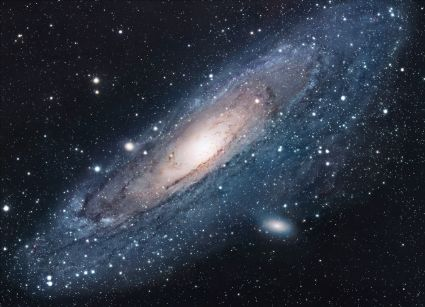
\includegraphics[scale=1.7]{universe}
%\caption{The Universe}
%\label{fig:universe}
%\end{figure}

%\section{Conclusion}
%``I always thought something was fundamentally wrong with the universe'' %\citep{adams1995hitchhiker}

%@article{einstein,
%    author =       "Albert Einstein",
%    title =        "{Zur Elektrodynamik bewegter K{\"o}rper}. ({German})
%        [{On} the electrodynamics of moving bodies]",
%    journal =      "Annalen der Physik",
%    volume =       "322",
%    number =       "10",
%    pages =        "891--921",
%    year =         "1905",
%    DOI =          "http://dx.doi.org/10.1002/andp.19053221004"
%}
 
%@book{latexcompanion,
%    author    = "Michel Goossens and Frank Mittelbach and Alexander %Samarin",
%    title     = "The \LaTeX\ Companion",
%    year      = "1993",
%    publisher = "Addison-Wesley",
%    address   = "Reading, Massachusetts"
%}
 
 
%\[E=mc^2\]
%\begin{equation}
%E=m
%\end{equation}

% Subscripts in math mode are written as $a_b$ and superscripts are written as $a^b$. These can be combined an nested to write expressions such as